\section{UI Toolkits}
\label{research:UIToolkits}
\textbf{Source:} \cite{PrimeVueVueUI} \cite{ShadcnVueShadcn} \cite{NaiveUIVue}
With Vue selected as my frontend framework I now wanted to research different ways of creating an aesthetically appealing UI design.

As noted previously Vue UIs are composed from components which in turn produce different views, for example this login page 
\begin{figure}[H]
    \centering
    
\includegraphics[width=0.6\textwidth]{Research/12_UIToolkits/media/loginPage.png}
    \caption{Example login page component}
\end{figure}

This Login page would be considered a single view, this view is composed from multiple elements which could potentially be: a data input element for email \& password (which themselves could be made from a box component and a text label component which is placed inside)

Whilst the official Vue documentation I read didn’t explicitly mention a preferred styling system I conducted many hours of research on platforms such as Stack Overflow, Reddit and YouTube to find the opinions of developers who don't just care about the final end product but the experience of developing with the platform. From this research I created the tables below



\begin{longtable}{%
  >{\raggedright\arraybackslash}p{0.18\textwidth}  % Framework
  >{\raggedright\arraybackslash}p{0.22\textwidth}  % Intro
  >{\raggedright\arraybackslash}p{0.20\textwidth}  % Positives
  >{\raggedright\arraybackslash}p{0.20\textwidth}  % Negatives
  >{\raggedright\arraybackslash}p{0.20\textwidth}  % Conclusion
}
\caption{Framework Evaluation Table} \\
\toprule
\textbf{Framework} & \textbf{Intro} & \textbf{Positives} & \textbf{Negatives} & \textbf{Conclusion} \\
\midrule
\endfirsthead

\toprule
\textbf{Framework} & \textbf{Intro} & \textbf{Positives} & \textbf{Negatives} & \textbf{Conclusion} \\
\midrule
\endhead

\midrule
\multicolumn{5}{r}{\emph{Continued on next page}} \\
\bottomrule
\endfoot

\bottomrule
\endlastfoot

% === Table content starts here ===

PrimeVue & 
PrimeVue is a popular UI component library specifically designed for Vue.js. It offers a comprehensive set of components with rich features and extensive documentation. &

- Wide variety of components with built-in themes and customization options.

- Strong community and excellent documentation.

- Regular updates and enterprise support.

- Works well with Vue 3’s composition API. &


- Styling is not as modern or flexible as Tailwind-based solutions.

- Can feel bloated for simple projects.

- Some components may have a steep learning curve for beginners. &

PrimeVue excels for enterprise projects and teams that need a full-featured, ready-to-use component set, but it lacks the modern design flexibility found in newer solutions and can be too rigid and complicated for solo developers who want to design more custom UIs. \\

Shadcdn & ShadCN is a modern, lightweight UI component collection for Vue and React, built on top of Tailwind CSS (a widely used styling system). It provides a clean, minimalistic design with a focus on accessibility and developer experience. Originally design to be used in React, it has recently been ported for use in Vue by the community &
 - Highly customizable with Tailwind CSS for seamless design consistency. 

- Lightweight and performant, avoiding unnecessary bloat.  

- Great DX (Developer Experience) with intuitive components. 

- Modern aesthetics and responsive by default.  

- Excellent accessibility support 'out of the box'

- Encourages a utility-first design approach, giving more flexibility. 

 - Active and growing community.

- All components are fully accessible for easy modification

& 
- Requires familiarity with Tailwind CSS for full customization.  

- Smaller component set compared to PrimeVue. 

- Less enterprise-grade support and documentation compared to older libraries.
& ShadCN is an excellent choice for developers seeking a modern, lightweight, and highly customizable UI framework, especially for those who prefer a Tailwind-based workflow. It’s perfect for building stylish and responsive apps efficiently. \\

Naive UI &  Naive UI is also a Vue only component library that provides a clean and elegant design with a focus on simplicity and flexibility. It’s known for its seamless integration with Vue’s reactivity system. & - Vue native with reactive components and seamless TypeScript support.  
- Modern design with customizable themes.

- Lightweight and modular, allowing selective imports. 

- Very performant.

& 
- Smaller community and ecosystem compared to PrimeVue.

 - Fewer components compared to larger frameworks.  

- Limited third-party integrations and ecosystem tools.

& Naive UI is a solid choice for Vue projects that need a lightweight yet feature-rich UI framework. However, it is not as versatile or widely supported as other library options.
\\
\end{longtable}


To conclude:
I believe Shadcdn will be the best choice for my project, whilst it hasn’t been as established as a Vue platform, the default components (see right) match my current visions for the project well and include a variety of tools built in a intuitive and (crucially) accessible way. The documentation is more sparse than other alternatives (especially for the Vue specific tools) however with the intuitiveness of the syntax and system design considered it seems to be a very developer friendly way of building a UI System

\begin{figure}[H]
    \centering
    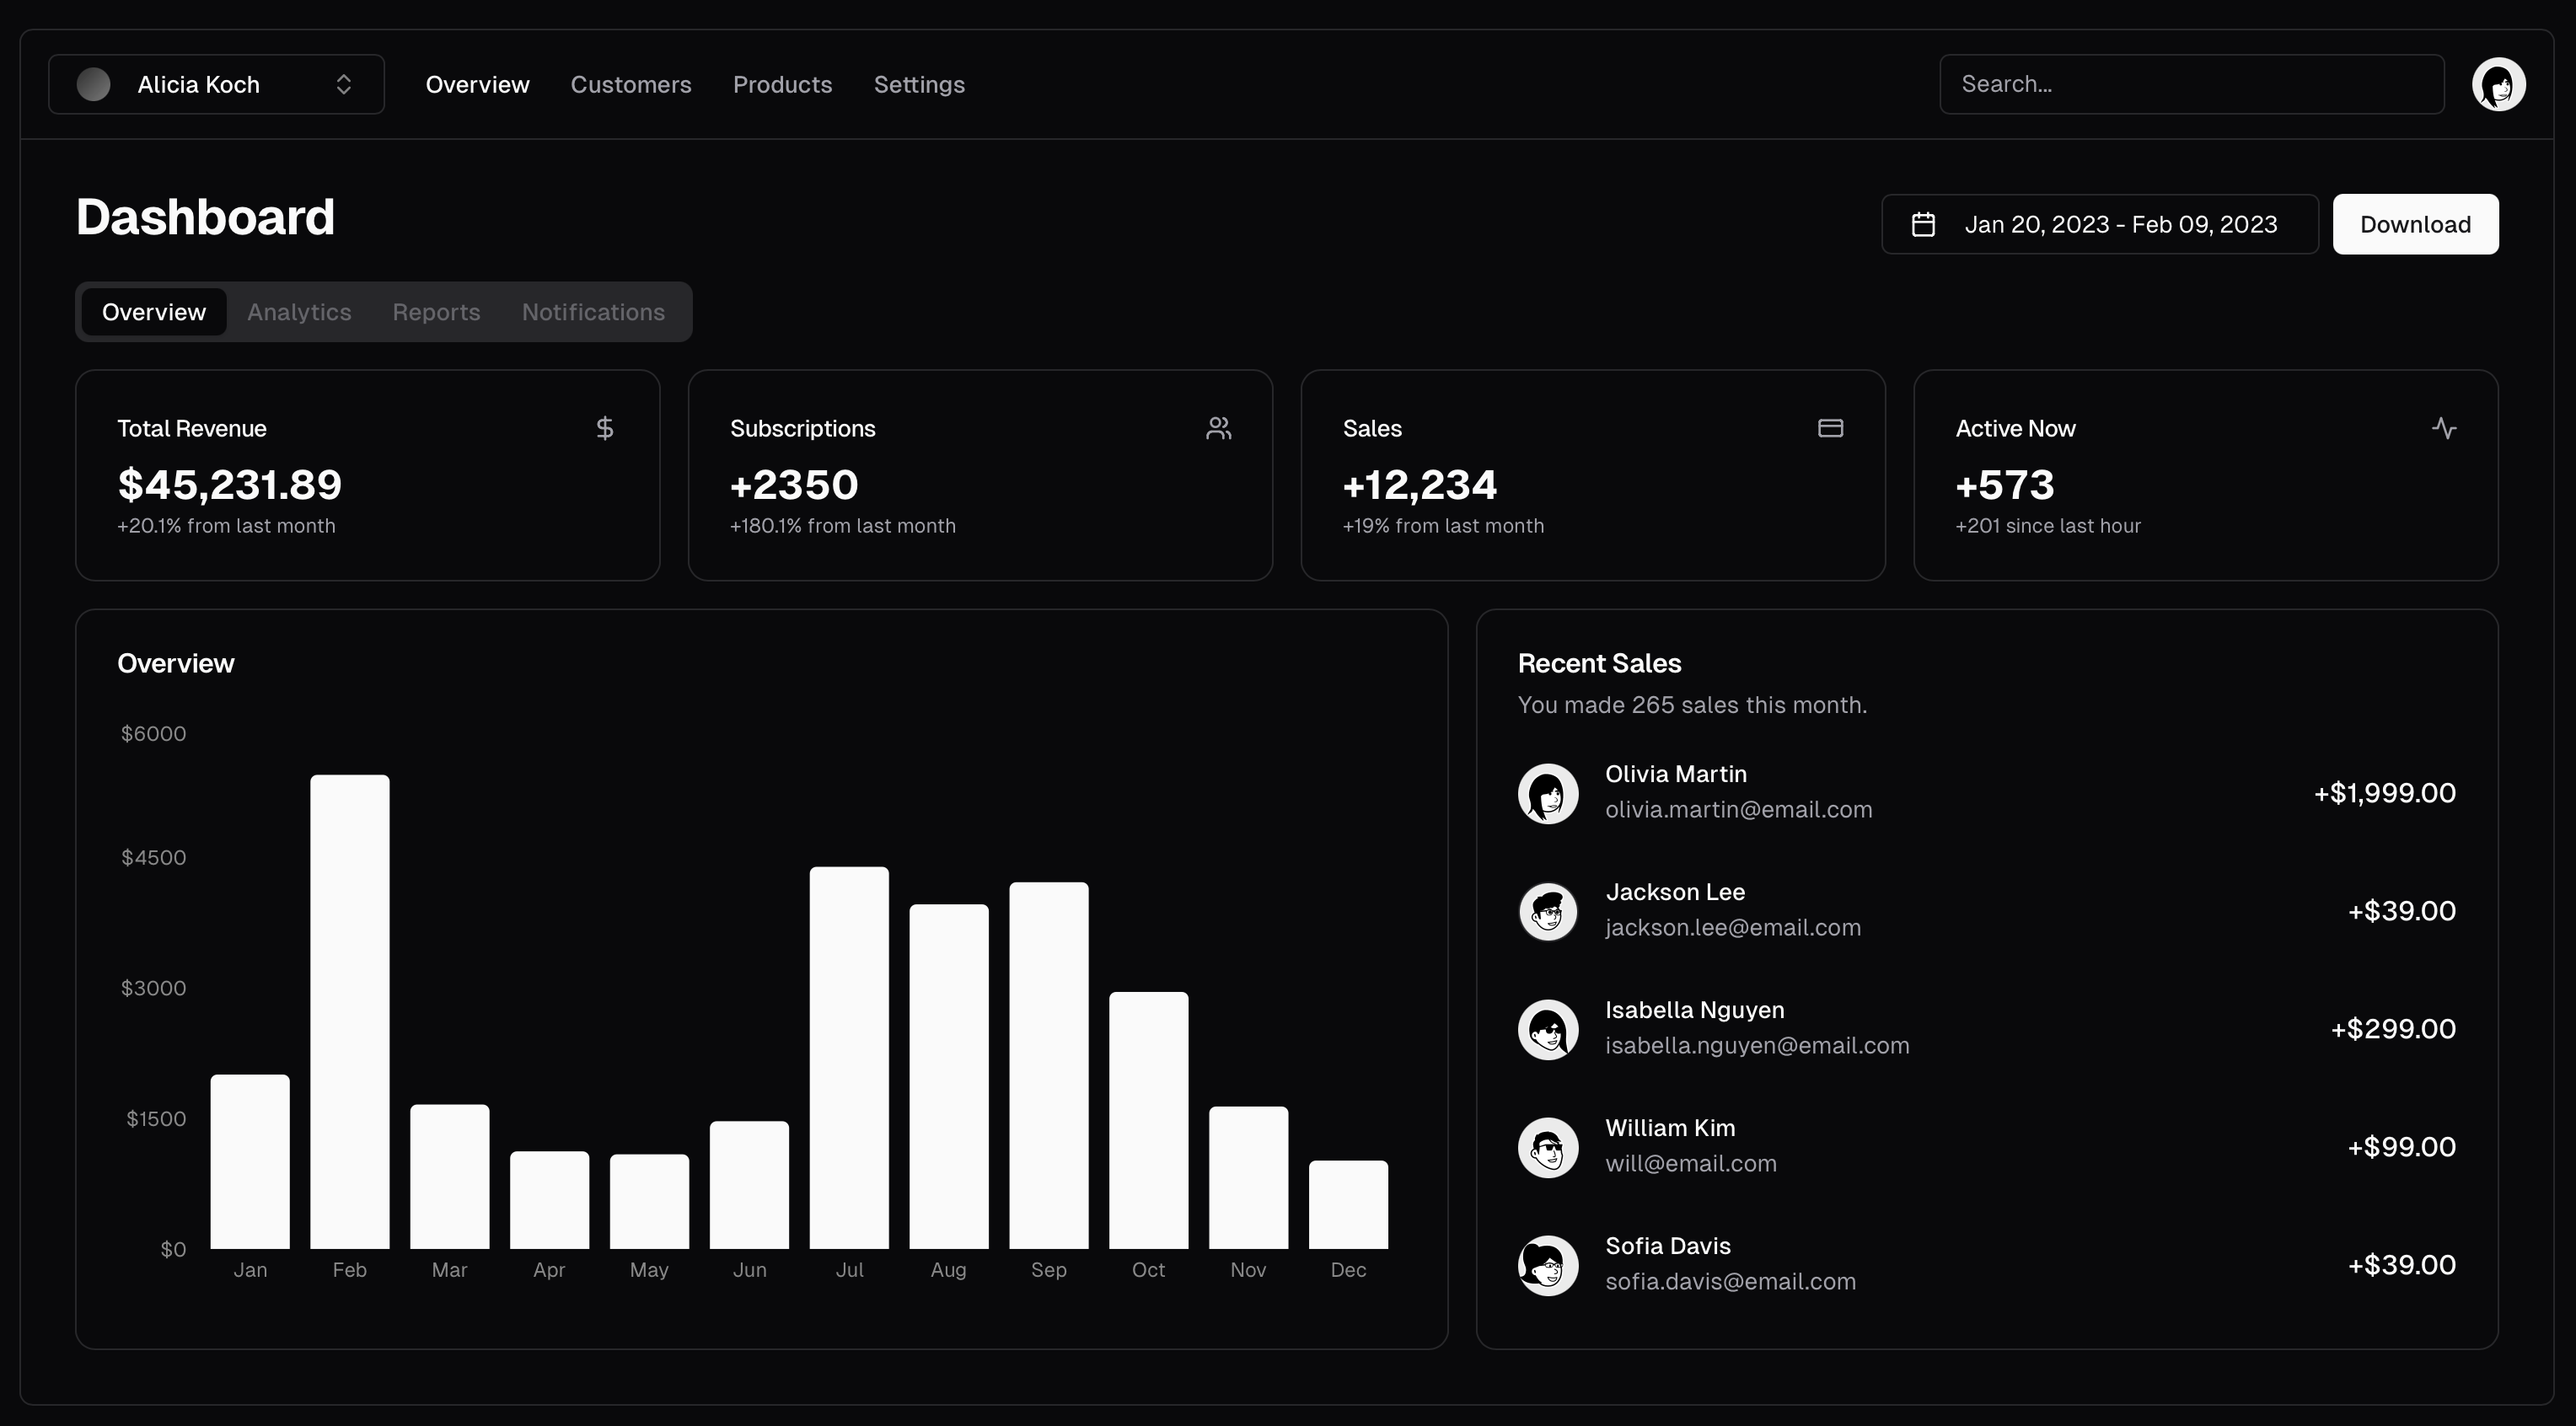
\includegraphics[width=0.6\textwidth]{Research/12_UIToolkits/media/Dashboard.png}
    \caption{Example Dashboard page code using Shadcn components}
\end{figure}

